% **************************************************
% Document class
% **************************************************

\documentclass[
	a4paper,
	12pt,
	bibliography=totoc,
	listof=totoc,
	titlepage
]{scrartcl}


% **************************************************
% Settings
% **************************************************

\usepackage{settings}


% **************************************************
% Variables
% **************************************************

\newcommand*{\getUniversity}{Hochschule für angewandte Wissenschaften München}
\newcommand*{\getFaculty}{Fakultät für Informatik und Mathematik}
\newcommand*{\getTitle}{Implementierung eines drahtlosen Fußschalters}
\newcommand*{\getAuthor}{Wolfram Barth}
\newcommand*{\getMatriculationNumber}{03708119}
\newcommand*{\getCourse}{Informatik}
\newcommand*{\getDoctype}{Bachelorarbeit}
\newcommand*{\getSupervisor}{Prof. Dr. Stefan Wallentowitz}
\newcommand*{\getSubmissionDate}{\today}


% **************************************************
% PDF Metadata
% **************************************************

\hypersetup{
	pdftitle = \getTitle,
	pdfauthor = \getAuthor,
	pdfsubject = \getDoctype
	pdfkeywords = {Bachelorarbeit, Informatik}
}


% **************************************************
% Content
% **************************************************

\begin{document}

\titlehead{
	\begin{flushright}
		
\includegraphics[width=50mm]{logos/university_logo}
	\end{flushright}
	\begin{center}
		{\Large \getUniversity}\\
		{\large \getFaculty}
		\vspace*{10mm}
	\end{center}
}

\subject{\getDoctype\ zum Thema:}

\title{\vspace{-10mm} \getTitle}

\subtitle{Zur Erlangung des akademischen Grades Bachelor of Science}

\author{}

\date{}

\publishers{
	\parbox{\textwidth}{
		\vspace*{40mm}
		\large
		\begin{tabularx}{0.8\textwidth}{lX}
			\textbf{Vorgelegt von:} & \getAuthor \\[0.7em]
			\textbf{Matrikelnummer:} & \getMatriculationNumber \\[0.7em]
			\textbf{Studiengang:} & \getCourse \\[0.7em]
			\textbf{Betreuer:} & \getSupervisor \\[0.7em]
			\textbf{Abgabedatum:} & \getSubmissionDate \\[0.7em]
		\end{tabularx}
	}
}\normalsize

\maketitle

\begin{abstract}

\section*{Abstract}
Die Digitalisierung von Hand- und Messwerkzeugen in der Industrie führt dazu, dass eine steigende Menge an Daten zusammengeführt und verarbeitet werden muss. Sie werden dazu in speziellen Formaten benötigt, weshalb entweder Software- oder Hardware-Lösungen für die Umwandlung von Nöten sind. Während die Software-Lösungen, aufgrund der hohen Sicherheitsrichtlinien in der industriellen Fertigung, zeitaufwändige und komplexe Einführungsprozesse nachsichziehen, gibt es noch keine Hardware-Lösungen, welche sowohl die Umwandlung in die benötigten Formaten, als auch die kabellose Anbindung des Hand- und Messwerkzeugen übernimmt. Dabei wird die folgende Forschungsfrage gestellt: Wie sollten die Software- und Hardware-Komponenten eines intelligenten Fußschalters gestaltet werden, damit dieser ohne die Installation weiterer Software Hand- und Messwerkzeug an ein Computersystem kabellose anbindet und deren Messergebisse in verschiedenen konfigurierbaren Formaten zur Verfügung stellt? Es wird auf einem intelligenten Fußschalter, als auch auf einem USB-Dongle, eine Anwendung entwickelt, welche die Daten von Messwerkzeugen zusammenführt und für die Weiterverarbeitung aufbereitet. Diese Anwendung stellt einen neuen softwarebasierten Ansatz da, wie industrielle Hand- und Messwerkzeug an einen Computer angebunden werden kann und die Messdaten verarbeitet werden können. Sie kann von der Industrie dazu verwendet werden um darauf aufbauend konkrete Produkte zu entwickeln. So wird die Hoffmann Group, für deren Werkzeug exemplarisch die Implementierung durchgeführt wurde, den Fußschalter und USB-Dongle in ihr Produktportfolio aufnehmen. Die Ergebnisse der Entwicklung werden evaluiert und werden von der Forschung dazu verwendet, um weitere Konzepte zur Anbindung von Werkzeugen an Computer zu entwickeln.

\end{abstract}

\tableofcontents

\clearpage
\listoffigures

\clearpage
\listoftables

\clearpage
\lstlistoflistings

\clearpage
\section*{Abkürzungsverzeichnis\markboth{Abkürzungsverzeichnis}{}}
\addcontentsline{toc}{section}{Abkürzungsverzeichnis}

\begin{acronym}[CI]

\acro{HCT}[HCT]{Hoffmann connected tools}
\acro{BLE}[BLE]{Bluetooth low energy}
\acro{HID}[HID]{Human interface device}
\acro{MSC}[MSC]{Mass storage class}
\acro{CSV}[CSV]{Comma seperated values}
\acro{CAQ}[CAQ]{Computer-aided quality assurance}
\acro{FIFO}[FIFO]{First in first out}
\acro{FAT}[FAT]{File allocation Table}
\acro{USB}[USB]{Universal Serial Bus}
\acro{UART}[UART]{Universal Asynchronous Receiver Transmitter}
\acro{LED}[LED]{light-emitting diode}
\acro{IDE}[IDE]{Integrated Development Environment}

\end{acronym}

\clearpage
\input{chapters/01_Einleitung}

\clearpage
\input{chapters/02_Ausgangszustand}

\clearpage
\input{chapters/03_Überarbeitung_des_bestehenden_Projekts}

\clearpage
\section{Einbindung Messuhren}
Mit dem Fußschalter soll ein Gerät geschaffen werden, dass die Messdaten von einem möglichst breiten Spektrum an Werkzeug sammeln kann. Dabei bestehen grundlegende Abhängigkeiten zum Medium der Verbindung (\ac{BLE}) und zum Protokoll (\ac{HCT}), das über diese Verbindung gesprochen wird. Diese werden aufgrund der Spezifikation des Fußschalters nicht aufgelöst. Jedoch soll für diese Geräte Mechanismen geschaffen werden, um sie möglichst vollständig einzubinden und für in Zukunft entwickelte Geräte erweiterbar zu bleiben. Dabei gilt es außerdem die oft sehr unterschiedlichen Funktionen der Geräte im Fußschalter zu vereinen.\\
Daher wird auch in Vorbereitung auf die Implementierung der fußschalterspezifischen Features die Dongle-App um die Unterstützung der Messuhren bzw. Messschieber erweitert. Messuhren und Messschieber sind in diesem Kontext dabei gleich bedeutend, weil das \ac{HCT}-Interface für beide Geräte identisch ist. Es wird sich nachfolgend jedoch stets auf Messuhren bezogen, da sie für die Anwendungsfälle des Fußschalters und Dongles bedeutender sind.

\subsection{Unterscheidung der Geräte}
Bei der Einbindung von neuen Geräten in die Anwendung des Fußschalters zeigt sich schnell ein grundlegendes Problem. Während das \ac{HCT}-Protokoll den Verbindungsaufbau vollständig abstrahiert und damit alle \ac{HCT}-fähigen Geräte verbunden werden können, bestehen in den darüber hinausgehenden Daten schwerwiegende Unterschiede.\\
Im einfachsten Anwendungsfall ist der Fußschalter mit mehren Werkzeugen verbunden und sammelt passiven deren Messergebnisse auf. Unabhängig vom eingestellten Messmodus benötigt die Dongle-App von den Geräten einerseits das Messergebnis und andererseits die Messeinheit, um die Ergebnisse vollständig an den Computer weitergeben zu können. Diese befinden sich abhängig vom Gerät an folgenden \ac{HCT}-Protokoll-Adressen:
\begin{table}[H]
	\centering
	\begin{tabular}[H]{l|l|l}
		 & Datenblock & Adresse \\
		\hline
		Garant Drehmomentschlüssel & & \\
		Messergebnis & Measurement data block & 0x00000B04 \\
		Messeinheit & Setpoint data block & 0x00000C1F \\
		\hline
		Holex Drehmomentschlüssel & & \\
		Messergebnis & Device measurement result & 0x0000240C \\
		Messeinheit & Device measurement case config & 0x0000221B \\
		\hline
		Messuhren/Messschieber & & \\
		Messergebnis & Device measurement result & 0x00002408 \\
		Messeinheit & Device measurement case config & 0x0000220F \\
		
	\end{tabular}
	\caption{Adressen Messergebnis und Messeinheit}
\end{table}
In Tabelle 1 wird deutlich, dass die Adressen von Messergebnis und Messeinheit für diese drei Geräte jeweils unterschiedlich sind, auch wenn sie im Fall der Messuhren und Holex Drehmomentschlüssel im gleichen Datenblock liegen. Wird dieser als Binärdaten erhalten kann die Adresse des Datenblocks gelesen werden, die Information von welchem Gerät die Daten stammen und damit an welcher Stelle genau die jeweils die Daten zu finden sind, kann jedoch nicht festgestellt werden. Es bleibt also keine andere Möglichkeit als die verbundenen Geräte ihrem Typ zuzuordnen und die erhaltenen Daten entsprechend zu interpretieren.\\ 
Diese Unterscheidung mit welcher Art von Gerät kommuniziert wird, kann auf zwei verschiedenen Weisen erfolgen. Einerseits kann anhand des Namens das Gerät entweder der Klasse Drehmomentschlüssel oder Messuhr zugeordnet werden. Das ist jedoch unter Umständen fehleranfällig, da das Sortiment an \ac{HCT}-Werkzeug stetig wächst und es nicht auszuschließen ist, dass in der Zukunft Geräte auf den Markt kommen, mit deren Namen es zu falschen Zuordnung kommt. Zudem gibt es alte Messschieber, die zwar unter einem korrekten Name advertisen aber nicht das \ac{HCT}-Protokoll sprechen, wobei diese Geräte aufgrund der Inkompatibilität der Protokolle letztendlich nicht verbunden werden sollten.\\
Eine andere Methode ist, die ``Device Information'' abzufragen und anhand der Klassenidentifikationsnummer das Gerät einem Typ zuzuordnen. Das ist die präferierte Lösung, da neben der genaueren und sicheren Zuordnung, in der Device Information andere Informationen, wie die Protokoll Version mitgeliefert werden, die bei späteren Features unter Umständen benötigt werden. Zudem bleibt die Datenverarbeitung leichter erweiterbar um neue Geräte. Jedoch muss diese Abfrage in den asynchronen und mehrteiligen Ablauf des Verbindungsaufbaus eingefügt werden, wodurch ein höherer Entwicklungsaufwand entsteht. Auch benutzen Drehmomentschlüssel der Firma Garant eine andere Klassifikation der Geräte als das Werkzeug der Firma Holex, welche innerhalb der Dongle-App vereinheitlicht werden muss.\\
Da die Erweiterbarkeit und Flexibilität jedoch dem höheren Entwicklungsaufwands überwiegen, wurde sich zugunsten dieser Lösung entschieden. Dabei wird nach dem Verbindungszustand-Callback, der vom Central Device nach einer erfolgreichen Subscription der Anwendung auf die \ac{BLE}-Charakteristik des Werkzeugs aufgerufen wird, eine Nachricht zu Abfrage der Device Information gesandt. Die erhaltenen Daten werden dann in der zum Gerät gehörenden Struktur gespeichert und anschließend die Abfrage der Messeinheit durchgeführt. Dies muss mithilfe eines Debuggers überprüft werden, da vorerst die Ausgabe der Messergebnisse von Messuhren nicht funktioniert. Dazu werden einen Drehmomentschlüssel und eine Messuhr mit einem nRF52840 DK development board verbunden. Dann kann mit dem Debugger der IAR-Workbench \ac{IDE} direkt die Werte in der Gerätestrukturen überprüft werden.
%TODO: Bild 

\subsection{Anpassung der Messdatenverarbeitung}
Auch die Datenverarbeitung, also die Interpretation der erhalten Daten über \ac{BLE} muss angepasst werden, da das Messergebnis, wie bereits in Tabelle 1 gezeigt, zwar innerhalb des gleichen Datenblocks wie bei dem Holex Drehmomentschlüssel liegt, jedoch innerhalb des Datenblocks an einer anderen Stelle. Diese Offsets sind als Konstanten im Headerfile der Dongle-App definiert und müssen um die entsprechenden Einträge für die Messuhren erweitert werden. Werden die Daten erhalten wird als Erstes die Adresse ausgelesen und dann je nach Typ des zugehörigen Geräts, die Interpretierung der Daten durchgeführt. Sollen also weitere Geräte eingebunden werden, können zusätzliche Sonderbehandlungen der Daten anhand des Typs hinzugefügt werden. Zudem handelt es sich bei dem Messergebnis, das von Interesse ist, beim Drehmomentschlüssel um den ``Peak Torque'', der als Gleitkommazahl codiert ist, während bei der Messuhr das Ergebnis die ``Measurement Distance'' als Ganzzahl codiert ist. Dabei handelt es sich abhängig von der Messeinheit um Mikrometer oder Mikroinch. Es muss auf Millimeter beziehungsweise Inch umgerechnet werden, da die Ausgabe über CDC oder \ac{HID} der Anzeige auf dem Gerätedisplay gleichen soll. Das binäre Messergebnis wird daher zunächst mit einem Umrechnungsfaktor von 1000 in Millimeter beziehungsweise Milliinch als Gleitkommazahl umgerechnet. Anschließend muss überprüft werden, ob es sich bei der derzeitige Einheit des Geräts um Inch handelt, da dann der Wert erneut durch 1000 dividiert werden muss, um von Milliinch auf die gewünschte Einheit Inch zu gelangen. Es wird also letztendlich eine Gleitkommazahl erhalten, wodurch sie ohne Anpassungen in der Nachrichten Struktur der Dongle-App gespeichert werden kann.\\
Die Einheitenkodierung der Messuhr ist komplementär zur Kodierung der Drehmomentschlüssel und daher kann die if-Cascade, welche die Zuordnung vornimmt, um die Einheiten der Messuhr erweitert werden. Jedoch befindet sich die Information welche Einheit verwendet wird, wie das Messergebnis, ebenfalls an einer anderen Stelle innerhalb des Datenblocks und muss entsprechend angepasst werden.

\subsection{Gruppenfunktion}
Zwischen Messuhren und Drehmomentschlüssel besteht ein funktioneller Unterschied. Zwar messen beide Geräte kontinuierlich einen Wert, jedoch ist das eigentliche Messergebnis, das ausgegeben und gespeichert wird ein jeweils anderes. Eine Messuhr oder Messschieber zeigt ausschließlich den derzeitigen Messwert an, während der maximal Wert in einer bestimmten Zeit von keinem Interesse ist. Das ist bei einem Drehmomentschlüssel genau anders herum, da er nachdem eine Schraube angezogen wurde, die maximal erreichte Kraft, die während der Verschraubung erreicht wurde, als Messergebnis anzeigen soll und es auch solange anzeigt, bis erneut eine Kraft am Drehmomentschlüssel anliegt. Die Funktionalität des Fußtasters den Anwender zu befähigen ein Messergebnis zeitgenau und präzise auszulösen, hat bei der Art wie das Messergebnis bei Drehmomentschlüssel vorliegt, keine besondere Bedeutung. Es wurde sich daher entschieden bei Betätigung des Fußtasters nicht das Messergebnis von Drehmomentschlüssel abzufragen, sondern die Funktionalität ganz auf Messuhren zuzuschneiden.\\
Durch das Betätigen des Fußtasters des Fußschalters soll bei allen verbundenen Messuhren das derzeitige Messergebnis abgefragt werden. Während im Modus 2 (CDC) ein Messergebnisse, anhand der Kanalnummer einem Werkzeug zugeordnet werden kann, ist dies in den \ac{HID}-Modi nicht der Fall. Es muss daher die korrekte Reihenfolge der Ausgabe der Messergebnisse sichergestellt werden. Es wurde sich entschieden, das devices.csv Konfigurationsfile um eine Spalte mit einer Gruppennummer zu erweitern, da somit der Anwender sowohl die Reihenfolge als auch welche Messuhren in der Gruppe sind, konfigurieren kann. Da durch das Abschicken der Nachrichten zur Abfrage der Messungen in der korrekten Reihenfolgen, das tatsächliche Erhalten in der gleichen Reihenfolge nicht sichergestellt ist, muss davon ausgegangen werden, dass die Nachrichten in einer zufälligen Reihenfolgen erhalten werden. Stattdessen muss bei der Ausgabe die Nachrichten umsortiert werden. Dazu bedarf es eines Zählers, der durch Betätigung des Fußschalters, von 0 auf 1 gesetzt wird, wodurch der Start der Gruppenfunktion später beim Erhalten der Messergebnisse erkennbar ist. Bei der Abarbeitung der erhaltenen Nachrichten, wird dann über die Zuordnung zum Device, die Nachricht ausgewählt und weitergegeben, die zum Counter korrespondiert. Die Gruppenids, die keinem der konfigurierten Geräte zugeordnet werden können, sowie die Gruppenids die zu unverbundenen Geräten gehören, werden dabei übersprungen. Zusätzlich soll ein Feature der Messeruhren genutzt werden, um die Gruppennummer auch auf der Messuhr anzuzeigen. Dazu werden den Messuhren ihre Gruppennummer nach dem Verbindungsaufbau via dem \ac{HCT}-Protokoll übermittelt.\\
Durch spätere Anregungen von Messtechnikern ergab sich jedoch, dass wenn ein Gerät der Gruppe zwar konfiguriert, jedoch nicht verbunden ist, die präferierte Lösung ist die gesamte Gruppe nicht zu triggern. Das ergibt sich einerseits dadurch, dass die Messuhren sich aufgrund ihrer relativ kleine Batterien bei Inaktivität schnell ausschalten und die Verbindung zu ihrem Central trennen. Anderseits soll möglichst jede durchgeführte Messung korrekt sein, da sie durch die \ac{CAQ}-Software verarbeitet und gespeichert wird. Das Ziel der Sicherstellung einer korrekten Messung überwiegt hier also dem Gedanken der Benutzerfreundlichkeit, dass eine Messung auch dann gemacht werden kann, wenn einer der Geräte unverbunden ist. Der Fußschalter blinkt dann zwei Mal kurz rot auf, um diesen Fehler zu signalisieren.\\
Des Weiteren könnte es passieren, dass eine Messung zwar angefragt, aber nicht erhalten wurde. Die Anwendung würde dann blockieren, da auf die Nachricht gewartet wird und müsste neugestartet werden. Es wurde sich entschieden, einen Timer zu starten, falls eine Nachricht nicht erhalten wurde und bei seinem Ablaufen statt dem Messergebnis eine Fehlermeldung auszugeben. Die restlichen Messergebnisse können dann korrekt ausgegeben werden.\\
Ebenfalls aus dem Feedback der Messtechnikern heraus, wurde ein sequentielles Triggern der Gruppe implementiert. Dazu muss der entsprechende Eintrag in der Konfigurationsdatei mit einer Eins auf aktiv gesetzt werden. Es wird bei den Geräten der Gruppe nacheinander, jeweils bei Betätigen des Fußtaster, die Abfrage des Messergebnis ausgegelöst.

\clearpage
\section{Einbindung Hardware}
Die Prototypen des Fußschalters der Firma Brecht wurden bereits vor Beginn dieser Arbeit erhalten und somit konnte direkt mit der Inbetriebnahme der neuen Hardware begonnen werden. Der Chipsatz des Fußschalters ist ebenfalls der PCA10056 von Nordic semiconductor, somit muss an der Software des USB-Dongles keine Änderungen vorgenommen werden.

\subsection{Energie Management}
Wenn der Fußschalter nicht über USB mit einer Stromquelle verbunden ist, bekommt er den benötigten Strom von dem fest eingebauten Akku. Um diesen nicht unnötig zu belasten, soll der Fußschalter nach einer Zeit der Inaktivität so weit wie möglich heruntergefahren werden.\\
Um diese Anforderung zu erfüllen, sah eine erste Idee vor das im nrf\_Base Projekt vorhandene Energiemanagement zu benutzen. Dieses fährt aus dem Main-Loop heraus getriggert den Chip bei Inaktivität des Softdevice weitestgehend herunter, wodurch der Stromverbrauch stark sinkt. Ist der USB-Port also nicht verbunden und es wurde keine Aktivität in der Fußschalter Anwendung, wie das Erhalten einer Nachricht oder dem Verbinden eines Geräts, registriert, wird ein Timer gestartet. Läuft dieser Timer ab, werden alle Central und Peripheren Verbindungen getrennt und falls notwendig Scanning und Advertising gestoppt. Wird während dem Laufen des Timers Aktivität registriert, wird er neugestartet, während er vollständig gestoppt wird, falls USB wieder verbunden ist. Dieser Implementierung lag die Vermutung zugrunde, dass wenn Chip vollständig heruntergefahren wurde, er auch nicht durch Betätigung des Fußtasters wieder neugestartet werden kann.\\
Zunächst zeigte sich jedoch das Problem, dass bei der Hardware des Fußschalters, der Akku auf der Datenleitung des USBs liegt. Dadurch wird in der Anwendung nicht wie bei dem EvalBoard die Events für USB connected und USB disconnect erhalten. Daher musste am Fußschalter geringfügige Hardwareänderungen durchgeführt werden. Dabei wurde die Eingangsspannung bereits vorher abgegriffen und auf den PIN des Fußtasters gelegt. Der Fußtaster erhält einen unbelegten PIN. Mit einem ADC wird dann überprüft, ob eine Spannung auf diesem PIN anliegt.\\
Es zeigte sich bei der Einbindung des Fußtasters, dass die Anwendung durch Betätigung des Fußtasters selbst aus einem Shutdown heraus wieder aufgeweckt wird. Daher wird nach Ablaufen des Inaktivitätstimers die Anwendung vollständig heruntergefahren, was noch energieeffizienter ist.

\subsection{Fußschalter Funktionalität}
Nach Überarbeitung der Codebasis und Einbindung der Messuhren, stehen alle Funktionalitäten bereit um den eigentlichen Fußtaster einzubinden. Während bei der initialen Einbindung des Fußtasters, eine Betätigung das Abfragen der Messergebnisse bei allen verbundenen Messuhren triggerte, wuchs die Funktionalität stetig.\\
Zum Ende dieser Arbeit wird durch ein kurzes Betätigen oder einem ``einfachen Klick'' die bereits beschriebene Gruppenfunktion ausgeführt. Im Modus 0 (USB-HID-singleKey) und 4 (BLE-HID-singleKey) wird draufhin ein Timer gestartet, welcher derzeit auf 500ms gesetzt ist. Wird während seines Laufen eine zweite Betätigung getätigt, wird ein ``Doppelklick'' registriert und das dafür in der Konfigurationsdatei hinterlegte Zeichen ausgegeben. Dadurch kann der User in diesem Modus schnell Dialogoptionen in der HCT-Windows-App auswählen oder in einem Textfile die Seiten wechseln. In einem anderen Modus führt das Warten auf die zweite Betätigung, jedoch zu einer Verzögerung der Ausgabe um die Dauer des Timers, weshalb dort die Doppelklick Funktionalität zugunsten dem Ansprechverhalten des Tasters gestrichen wurde.\\
Wird der Taster hingegen für 3 Sekunden durchgängig gehalten, wird das Gerät heruntergefahren. Diese Funktionalität wurde ursprünglich eingeführt, da der Fußschalter auf einer Messe vorgestellt wurde, aber der automatische Reset des Geräts bei Änderung der Konfigurationsfiles noch nicht zuverlässig funktionierte. Sie wurde beibehalten, da sie als sehr benutzerfreundlich empfunden wurde.

\subsection{Inbetriebnahme LED}
Auf dem Board des Fußschalters befindet sich eine LED die durch einen Lichtkanal nach außen hin durch das Gehäuse sichtbar gemacht wird und die dazu benutzt werden soll den internen Zustand des Geräts darzustellen. Folgende Zustände sollen abgebildet werden: 

\begin{table}[H]
	\centering
	\begin{tabular}[H]{l|l}
		Zustand & LED-Farbe \\
		\hline
		Gerät im Sleep Modus & Aus \\
		\hline
		Alle zu verbindenden Geräte verbunden & Blau \\
		\hline
		Min. ein Gerät verbunden, es wird nach den fehlenden Geräten gescannt & Blau blinkend \\
		\hline
		Kein Gerät verbunden, Scanning inaktiv & Grün \\
		\hline
		Kein Gerät verbunden, Scanning aktiv & Grün blinkend \\
		\hline
		MSC-Schreibvorgang detektiert & Gelb \\
		\hline
		Min. ein Konfigurationsfile nicht gefunden & Rot \\
		\hline
		Fehler in den Konfigurationsfiles & Rot blinkend \\
	\end{tabular}
	\caption{LED-Zustände}
\end{table}

\clearpage
\section{Messmodi}
Die durch den Fußschalter gesammelten Daten sollen in einem möglichst breiten Spektrum zur Weiterverarbeitung bereitgestellt werden. Auch durch den Fußtaster gegebene Funktionalitäten, wie aus das Ausgeben eines spezifischen und konfigurierbaren Zeichens bei Betätigung, soll abgedeckt werden. Der Anwender muss die Art wie der Fußschalter eingesetzt werden soll, spezifizieren können und die Datenverarbeitung innerhalb der Anwendung des Fußschalters muss dementsprechend flexible und anpassbar gestaltet werden. Eine weitere Herausforderung dabei ist, das dem Anwender nur äußerst begrenzte Interaktionsmöglichkeiten mit dem Fußschalter zu Verfügung stehen.\\
Um diesen Anforderungen gerecht zu werden, wurde sich entschieden Messmodi einzuführen. Dieser kann in einer zusätzlichen globalen Konfigurationsdatei angegeben werden und legt fest welche Funktionalität durch den Fußschalter bereitgestellt wird. Es folgt dem bereits bei der Konfiguration der zu verbindenden Geräte verwendeten Schema, dass das Gerät durch die Dateien die im Massenspeichermedium liegen konfiguriert wird und liefert dem Anwender visuelles Feedback über die derzeitigen Einstellungen. Durch Kommentare in der Konfigurationsdatei können zudem die möglichen Einstellungsoptionen dem Anwender leicht zugänglich gemacht werden.\\
Eine grundlegend andere Möglichkeit verschiedenste Einstellungen durchzuführen, ist es durch Kombinationen aus langen und kurzen Betätigungen des Fußtasters Menüs aufzurufen und mit Hilfe eines Bedienungsanweisung die gewünschten Optionen auszuwählen. Auch wenn diese Möglichkeit in Produkten wie Kaffeemaschinen oder digitalen Weckern eine weite Verbreitung findet, hat sie den entscheidenden Nachteil, dass der Anwender keinerlei grafisches Feedback bekommt. Auch ist es hierfür von Vorteil, wenn das Gerät mehrere Tasten besitzt um die Wahrscheinlichkeit des versehentlichen Ansteuern von Menüs und Umkonfiguration des Fußschalters zu minimieren.\\
Aufgrund des grafischen Feedbacks und der Konsistenz mit der Konfiguration der zu verbindenden Geräte wurde sich für die erste Möglichkeit dazu entschieden. Zum Zeitpunkt der Implementierung der Dongle-App war die App die oberste Abstraktionsschicht aller USB-Funktionalität. Das ist mit Einführung der Messmodi nicht mehr der Fall. Daher bedarf es einer neuen Abstraktionsschicht, die über der Dongle- und Fußschalterapp steht und die die verschiedenen Funktionalitäten dirigiert. Dadurch können die Operationsmodi programmatisch getrennt werden, sodass bestimmte Schritte der Initialisierung, wie das Einlesen der Konfigurationsdatei der zu verbindenden Geräte, in einem Modus wie \ac{HID} einzelnes Zeichen nicht ausgeführt werden. Außerdem bleibt die Anwendung dadurch leicht um neue Messmodi erweiterbar. Zum Ende dieser Arbeit sind folgende Modi konfigurierbar:
\begin{itemize}
	\item 0: USB-\ac{HID}-singleKey
	\item 1: USB-\ac{HID}
	\item 2: CDC (COM-Port)
	\item 3: \ac{BLE}-\ac{HID}
	\item 4: \ac{BLE}-\ac{HID}-singleKey
\end{itemize}

\begin{figure}[H] 
	\centering
	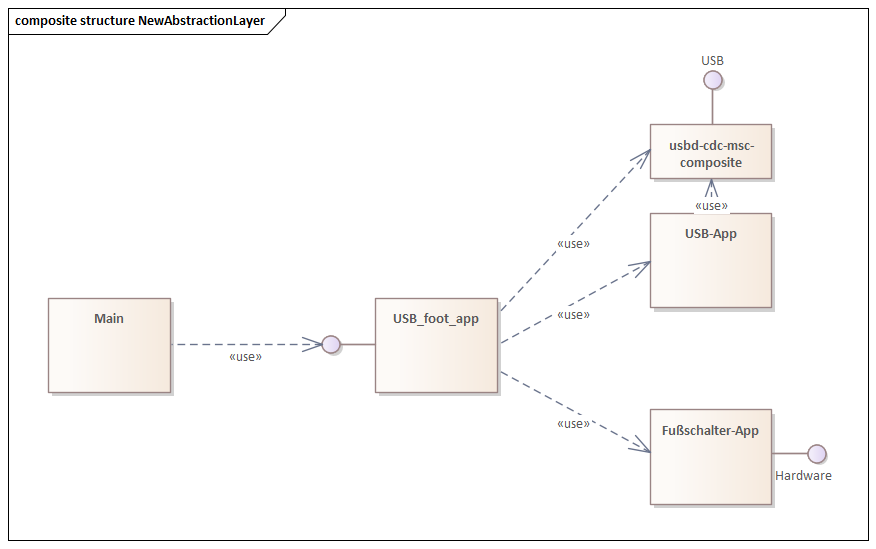
\includegraphics[width=\textwidth]{figures/NewAbstractionLayer.png}
	\caption{Neue Abstraktionsschicht}
\end{figure}

\subsection{USB-HID}
Ein Feature, das sowohl für den Dongle als auch für den Fußschalter implementiert werden soll, ist das Human Interface Device (HID) über USB. In diesem Modus gibt die Anwendung die Messergebnisse nicht mehr über den virtuellen COM-Port aus, sondern ist über USB als Tastatur mit dem Computer verbunden. Über sie werden die Zeichen der Messung als Tastendrücke, gefolgt von einem konfigurierbaren Terminierungszeichen, ausgegeben. Dadurch können Messungen einfach in Excel oder einem Texteditor aufgefangen werde.\\
Für die Implementierung werden die Funktionen des NRF-Library Files app\_usb\_hid\_kbd.h verwendet. Es abstrahiert die Low-Level USB-Aufrufe und stellt Funktionen zur Verfügung, die bei Aufruf eine Taste drücken oder loslassen. Es fehlt jedoch eine Funktion die ganze Strings serialisiert, weshalb diese implementiert werden muss. Die Scancodes, die Nummern der Tasturtasten, sowie der Modifier, eine Taste die Tastendrücke modifiziert, wie die Shift-Taste, werden dabei von einer Funktion erhalten, die im nrf\_Base Projekt enthalten ist. Sie wurde für die \ac{HID} Implementierung über \ac{BLE} geschrieben und gibt den Scancode und zugehörigen Modifier für einen ASCII Character zurück.\\
Zwischen den Tastendrücken muss eine gewisse Zeit gewartet werden, da der Computer Tastendrücke zwischen denen zu wenig Zeit verstreicht nicht registriert. Dieser Delay wurde auf 1 Millisekunden festgelegt, da bei einem längeren Delay die Anzahl an fehlerhaften Tastendrücken zunahm. Diese Art darauf zu warten, dass die Tastendrücke vom Computer registriert wurde, stellte sich jedoch als sehr fehleranfällig heraus. Nicht nur wurde dopplete Zeichen nicht korrekt erkannt, sondern nach ungefähr 10 Ausgaben schien der USB-Bus überlastet zu sein. Daher musste die Implementierung geändert werden. Statt die Tastendrücken ohne Rücksicht auf die zugehörigen Events dem USB zu übergeben, muss nach jedem Zeichen auf ein Event der USB-\ac{HID} Library gewartet werden, das die erfolgreiche Übertragung signalisiert. Dazu muss der zu serialisierende String in einem Buffer hinterlegt und bei Empfangen des Events das nächste Zeichen übertragen werden.\\
Eine Abwandlung dieses Modus, ist der Modus USB-\ac{HID}-singleKey. In diesem Modus gibt der Fußschalter bei Betätigung des Tasters nur ein einzelnes kofigurierbares Zeichen aus, beziehungsweise bei einem Doppelklick ein Zweites, wie in Abschnitt 5.2 beschrieben ist.

\subsection{BLE-HID}
Ein weiterer Modus, in dem der Fußschalter arbeiten soll, ist \ac{HID} über \ac{BLE}. Dabei simuliert der Fußschalter oder Dongle eine über \ac{BLE} verbindbare Tastatur und serialisiert nach dem Verbinden wie bei \ac{HID} über USB die Messergebnisse als Tastendrücken. Dazu muss das Gerät nun zusätzlich zur Central Rolle in der Peripheral Rolle agieren. Dazu muss einerseits das Advertising korrekt konfiguriert werden und in den bestehenden Code des Peripheren Verbindungsaufbaus, die Fußschalter Applikation eingebunden werden. Für das eigentliche Schreiben des Messergebnisses über \ac{BLE}, gibt es bereits eine bestehenden Funktionen des nrf\_Base Projekts die einen String vollständig serialisiert und diese muss nur in der Fußschalter Applikation aufgerufen werden.\\
Dabei erfordert dieser Modus es nun, dass die Bonding Informationen der Verbindung von Fußschalter zu Computer gelöscht werden kann. Werden sie nicht gelöscht, jedoch auf dem Computer, können sich die beiden Geräte nicht mehr miteinander verbinden. Das muss zum Beispiel geschehen, wenn der Fußschalter mit einem anderen Computer verbunden werden soll, sich der erste Computer jedoch noch in Reichweite befindet. Trotzdem sollen nicht bei jedem Reset des Fußschalter, also bei einer Änderung der Konfigurationsdatei, die Bonding Informationen gelöscht werden, da sonst bei jedem Verbinden, der Fußschalter im Computer erst entkoppelt und dann wieder neugekoppelt werden muss. Es kann also nicht direkt gesagt werden wann die Bonding Informationen gelöscht werden sollen und wann nicht, stattdessen wäre der Idealfall, dass der User selbst die Informationen löschen kann. Das ist jedoch aufgrund der begrenzten Interaktionsmöglichkeiten des Users mit dem Fußschalter nur schwierig umsetzbar. Ein Kompromiss ist, dass die Bonding Informationen gelöscht werden, wenn der Modus \ac{BLE}-\ac{HID} verlassen wird. Der Anwender kann dann auch um die Bonding Informationen zu löschen aus dem Modus 3 herauswechseln und dann wieder hineinwechseln. Dabei ist das Problem, dass bei einem Reset nicht direkt ersichtlich ist, in welchen Modus gewechselt wird, da die Konfigurationsdatei erst beim Neutstart neugelesen wird. Daher wird direkt vor dem Reset die Konfigurationsdatei gelesen und falls aus dem Modus 3 oder 4 in einen anderen Modus gewechselt wird, die Bonding Informationen gelöscht. Ein alternativer Lösungansatz der ohne das ressourcenfordernde Einlesen der Datei auskommt, ist die Bonding Informationen immer zu löschen, wenn sich der Fußschalter beim Reset in einem anderen Modus als 3 oder 4 befindet. Jedoch war dann der ``Peer Manager'' nicht initialisiert, der zum Löschen der Bonding Informationen zwingend benötigt wird, weshalb doch der erste Lösungansatz umgesetzt wurde. Der Peer Manager ist dabei eine Library von NRF die sich um Verschlüssung, Pairing und Bonding kümmert (\cite[]{NRF_PeerManager}).\\
Erste Tests zeigen, dass die Geschwindigkeit der Übertragung, einerseits die Dauer bis zum ersten Tastendruck und anderseits die Zeit zwischen den einzelnen Tastendrücken, zu hoch ist. Die Untersuchung wo genau zuviel Zeit verwendet wird, fand mithilfe eines Oszilloskop und dem togglen eines freien Pins, der zu diesen Debugzweck belegt wurde, statt. Es konnte dadurch bereits ein Bug im nrf\_Base Projekt gefunden werden. Dabei wird in der Funktion, zwischen den einzelnen Zeichen eine Pause gemacht, um ähnlich im Modus USB-\ac{HID} dem Betriebssystem Zeit zu geben die Tastendrücke zu verarbeiten. Dieser Delay ist abhängig von Connection Interval, welches wenn nur die Verbindung zum Computer besteht, korrekt gesetzt ist. Jedoch stellte sich heraus, dass diese globale Variable von allen Verbindungen stets überschrieben wird. Dabei ist diese Variable auch unabhängig von der \ac{HID} Funktionalität nur für die peripheren Verbindungen von Bedeutung und dieses Verhalten ein Fehler. Es wurde daher an der Stelle, an der diese Variable durch einen ``Connection Update Request'' überschrieben wird, die Unterscheidung eingeführt, ob es sich bei der Verbindung um eine periphere Verbindung handelt.\\
Auch von diesem Modus, gibt es die Abwandlung \ac{BLE}-\ac{HID}-singleKey, die wie im Modus USB-\ac{HID}-singleKey, ein einzelnes Zeichen bei Betätigung des Tasters ausgibt.


\subsection{BLE-HCT-Windows-App}
Der letzte Modus, in dem der Fußschalter agieren soll, ist als ein an die \ac{HCT}-Windows-App angebundenes Gerät. Dabei soll das Signal der Betätigung des Tasters als eine \ac{HCT}-Nachricht an die Windows-App gesendet werden, welchen dann ein Messergebnis bei den mit ihr verbundenen Messgeräten triggert. Dazu muss ein \ac{HCT}-Model für den Fußschalter geschaffen werden. Das Model stellt folgende Werte bereit:
\begin{itemize}
	\item Device Class
	\item Protocol type, version 
	\item Version of Hardware, Software, \ac{BLE}
	\item Battery level, status
	\item Reset 
\end{itemize}

Werte des Config.ini Konfigurationsfiles:
\begin{itemize}
	\item Operating Mode 
	\item CDC protocol 
	\item HID Keyboard Language ID 
	\item HID data set seperator 
	\item HID number seperator
	\item HID single key 
\end{itemize}

Für die Übertragung des eigentlichen Signals, dass der Fußschalter betätigt wurde, muss eine \ac{HCT}-Charakteristik angelegt werden, auf welche die \ac{HCT}-Windows-App sich subscriben kann. Über diese Charakteristik wird sie dann über die Betätigung des Tasters notifiziert. Im Advertising muss sich der Fußschalter dann nicht als Tastatur, sondern als \ac{HCT}-Fußschalter erkenntlich zeigen.\\
Es wurde jedoch beschlossen, diesen Modus erst in einer späteren Version des Fußschalters zu implementieren, wie im Abschnitt 8.2 genauer erklärt wird.

\clearpage
\input{chapters/07_ÜberarbeitungMSC}

\clearpage
\section{Schlusswort}

\subsection{Stand Produktentwicklung}
Der Fußschalter und der Dongle sollen als eigenständige Produkte in das Sortiment übernommen werden. Sie werden jeweils als Projekte von dem Produktmanagement übernommen. Dabei werden die Hardwareänderungen wie in Kapitel 5.1 beschrieben, in das Layout der Platine übernommen. Zusätzlich soll der Pin, der den Chip in den Bootloader Mode versetzt, von außen erreichbar gemacht werden. Außerdem sollen auch die SWE-Pads, die das Debugging auf dem Chip ermöglichen erreichbar gemacht werden. Derzeitig sind sie auf der Seite mit der der Dongle auf die Platine gelötet wurde, weswegen sie nur sehr schwer abgreifbar sind. Die Prototypen dieser neuen Hardwareversion wurden Anfang August erhalten.\\
Der Modus BLE-Windows-App wurde auf eine spätere Version verschoben, da die Integration der Messuhren in die Windows App andauert und eine Integration des Fußschalters daher noch nicht absehbar ist. Dieser Modus wurde zugunsten anderer Features bis auf Weiteres verschoben. 

\subsection{Fazit}
Der Implementierungsumfang für diese Arbeit war von Anfang an ambitioniert. Dennoch wurde alle geplanten Features außer der Modus BLE-Windows-App implementiert und sogar noch zahlreiche zusätzliche Features, wie die Gruppenfunktion, umgesetzt. Eine weiterführende Optimierung des Modus BLE-HID steht noch aus, aber steht einer Produkteinführung nicht im Weg.

\clearpage
\printbibliography

\clearpage
\begin{abstract}

\section*{Selbstständigkeitserklärung}
Hiermit erkläre ich, dass ich die Bachelorarbeit selbständig verfasst, noch nicht anderweitig für Prüfungszwecke vorgelegt, keine anderen als die angegebenen Quellen oder Hilfsmittel benutzt sowie wörtliche und sinngemäße Zitate als solche gekennzeichnet habe.\\

\bigbreak
\bigbreak

München, den \today

\end{abstract}

\end{document}